\documentclass[8.01x]{subfiles}
\begin{document}

\chapter{Week 7: Homework 6}

\section{Problem 1: Two blocks and a spring}

\begin{center}
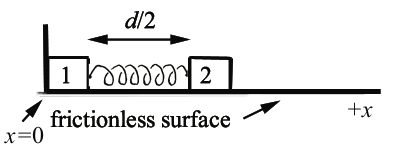
\includegraphics[scale=0.6]{Graphics/h6p1}
\end{center}

``A system is composed of two non-identical blocks connected by a spring. The blocks slide on a frictionless plane. The unstretched length of the spring is $d$. Initially block 2 is held so that the spring is compressed to $d/2$ and block 1 is forced against a stop as shown in the figure above. Block 2 is released.

Which of the following statements is true? (Note: more than one statement may be true.)

(a) When the position of block 2 is $x_2 > d$, the center of mass of the system is accelerating to the right.\\
(b) When the position of block 2 is $x_2 > d$, the center of mass of the system is moving at a constant speed to the right.\\
(c) When the position of block 2 is $x_2 > d$, the center of mass of the system is at rest.\\
(d) When the position of block 2 is $x_2 < d$, the center of mass of the system is accelerating to the right.\\
(e) When the position of block 2 is $x_2 < d$, the center of mass of the system is moving at a constant speed to the right.\\
(f) When the position of block 2 is $x_2 < d$, the center of mass is at rest.''

All right, let's see. The spring is compressed, so as we start this experiment, block 2 will accelerate towards the right. The blocks are ``non-identical'', so we can't say anything qualitative about the center of mass, other than that it must be somewhere between the blocks (possibly part-way inside one of them).

This is an easy problem, IF you approach it correctly. If you don't, it's very easy to get it wrong. The approach that is way easier than the others is to consider conservation of momentum. In the beginning of the problem, there is a net external force on the system -- the normal force from the wall pushing towards the right. Net force means acceleration, so to begin with, there is an \emph{acceleration towards the right}, while $x_2 < d$ (the spring is compressed), so option (d) is correct.

When block 2 passes $x_2 > d$, the spring starts to pull together, which moves block 1 towards the right. When it moves away from the wall, there is \emph{no longer a net external force} in the horizontal direction, and we can (and should) apply the conservation of momentum to consider what may happen next. No matter what the masses of the two blocks are, momentum must be conserved!

The net momentum of the system is $p_{tot} = m_{tot} v_{cm}$. The mass is not changing, and $p_{tot}$ must be held constant and so $v_{cm}$ \emph{is a constant} after this; option (b) is also correct. All options except (b) and (d) are thus incorrect.

This was demonstrated in lecture, with an extremely similar system, of two air track-carts and a spring. After the system had been set in motion, the center of mass held a constant velocity, despite the oscillating behavior of the two masses. That is exactly what will happen here.

Since the center of mass will hold a constant velocity towards the right, the system will keep moving towards the right until it hits an obstacle (given that we ignore friction).

\section{Problem 2: Pushing a baseball bat}

``The greatest acceleration of the center of mass of a baseball bat will be produced by pushing with a force $F$ at

(a) Position 1 (at the handle)\\
(b) Position 2 (at the center of mass, around the middle of the bat)\\
(c) Position 3 (at to the very edge)\\
(d) Any point. The acceleration is the same.\\
(e) Not enough information is given to decide.''

Honestly, I find this a bit nonintuitive, based an experience -- but it's important to note the force $F$ is the same in all cases.

We have found previously that the momentum of a system can be found as $m \vec{v_{cm}}$, where $m$ is the total mass:

\begin{equation}
\vec{p_{tot}} = m_{tot} \vec{v_{cm}}
\end{equation}

If we take the time derivative of this equation, we find

\begin{equation}
\frac{d p_{tot}}{dt} F_{ext} = m_{tot} \vec{a_{cm}}
\end{equation}

The change in momentum of the entire system is the same as the net external force, which is the same as the mass-acceleration product of the center of mass. That gives us, for the acceleration, $\displaystyle a_{cm} = \frac{F_{ext}}{m_{tot}}$. If $F = F_{ext}$ is constant, as it is, and $m_{tot}$ is also constant, then clearly the only possible answer is that the acceleration is the same for all points, the fourth option.

\url{http://www.youtube.com/watch?v=vWVZ6APXM4w} has a great demonstration of this effect. Make sure you watch the follow-up video \url{http://www.youtube.com/watch?v=N8HrMZB6_dU} and the explanation video \url{http://www.youtube.com/watch?v=BLYoyLcdGPc} too. They are a bit less than 15 minutes combined, but the effect is quite nonintuitive and so the videos are rather interesting.

\section{Problem 3: Jumping off the ground}

``A person of mass $m$ jumps off the ground. Suppose the person pushes off the ground with a constant force of magnitude $F$ for $T$ seconds.

What was the magnitude of the displacement of the center of mass of the person while they were in contact with the ground? Express your answer in terms of $m$, $F$, $T$, and $g$ as needed.''

Well, let's see. Since the force is constant, the impulse is simply given by $F T$. However, I think we should solve this is a different manner than impulse.

The movement of the center of mass is given by $F_{ext} = m a_{cm}$. With a constant force, and thus a constant acceleration, we can use $\Delta y = \frac{1}{2} a t^2$, with $a = a_{cm}$ and $t = T$.\\
However, let's not forget about gravity. $F_{net} = F - m g$, so $a_{cm} = F/m - g$. That gives us, for the displacement

\begin{equation}
\Delta y = \frac{1}{2} (\frac{F}{m} - g) T^2
\end{equation}

\section{Problem 4: Exploding projectile}

``An instrument-carrying projectile of mass $m_1$ accidentally explodes at the top of its trajectory. The horizontal distance between launch point and the explosion is $x_m$. The projectile breaks into two pieces which fly apart horizontally. The larger piece, $m_3$, has three times the mass of the smaller piece, $m_2$. To the surprise of the scientist in charge, the smaller piece returns to earth at the launching station. Neglect air resistance and effects due to the earth's curvature.

\begin{center}
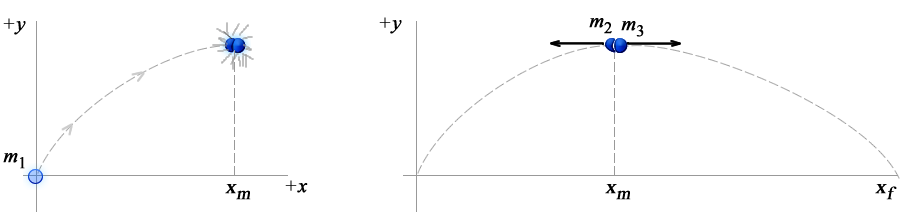
\includegraphics[scale=0.6]{Graphics/h6p4}
\end{center}

How far away, $x_f$, from the original launching point does the larger piece land? Express your answer in terms of some or all of the given variables $m_1$, $x_m$, and $g$.''

First, just in case we need them, let's write $m_2$ and $m_3$ in terms of $m_1$:

\begin{align}
m_2 &= \frac{m_1}{4}\\
m_3 &= \frac{3 m_1}{4}
\end{align}

Okay, so what do we know? Ignoring air drag, momentum is conserved in the $x$ direction. After the explosion, $m_2 v_2^{'} + m_3 v_3^{'} = m_1 v_1$.\\
$v_1 = x_m/t$, but we don't know $t$. However, we do also know (see below) that $v_2^{'} = - v_1$.

The smaller piece has a certain momentum after the launch, and the exact opposite momentum the other way back. Why? Because $p = m v$, and since it returns to exactly its launch point along the same path, the $v$ must be the same both ways, only in opposite directions. With no air drag, it takes the same amount of time to fall from the top down to the ground, and it must traverse the same horizontal distance back as it did in getting to the top during that same time, which implies having the same horizontal velocity, which for a given mass implies the same momentum (as far as magnitude goes).

The time $t$ taken for $m_3$ to hit the ground is exactly the same as that of $m_2$, since there is no air drag that could cause any difference in timing. Using conservation of momentum (equation one), substituting in $v_1 = x_m/t$ (equation two), substituting in the masses (equation three) and finally substituting in $v_3^{'} = (x_f - x_m)/t$:

\begin{align}
-m_2 v_1 + m_3 v_3^{'} = m_1 v_1\\
-m_2 (\frac{x_m}{t}) + m_3 v_3^{'} = m_1 \frac{x_m}{t}\\
-\frac{m_1}{4} (\frac{x_m}{t}) + \frac{3m_1}{4} v_3^{'} = m_1 \frac{x_m}{t}\\
-\frac{m_1}{4} (\frac{x_m}{t}) + \frac{3m_1}{4} \frac{(x_f - x_m)}{t} = m_1 \frac{x_m}{t}
\end{align}

All that remains is simplification. First we can eliminate $t$, followed by $m_1$ and multiplying it all by $4$:
\begin{align}
-\frac{m_1}{4} (x_m) + \frac{3m_1}{4} (x_f - x_m) = m_1 x_m\\
-(x_m) + 3 (x_f - x_m) = 4 x_m\\
\end{align}

And the remainder doesn't need much explanation:
\begin{align}
3 x_f &= 8 x_m\\
x_f &= \frac{8}{3} x_m
\end{align}

Just as I hoped, all terms could be written in terms of $t$, so that it could be eliminated, leaving only known values $m_1$ (which also cancelled) and $x_m$, plus the unknown $x_f$.\\
Quite a nice result!

\section{Problem 5: Center of mass of the Earth-Moon system}

``The mean distance from the center of the earth to the center of the moon is $r_{em} = \SI{3.84e8}{m}$. The mass of the earth is $m_e = \SI{5.98e24}{kg}$ and the mass of the moon is $m_m = \SI{7.34e22}{kg}$. The mean radius of the earth is $r_e = \SI{6.37e6}{m}$. The mean radius of the moon is $r_m = \SI{1.74e6}{m}$.

How far from the center of the earth is the center of mass of the earth-moon system located?''

We choose a coordinate system centered at the center of the Earth, which is clearly the simplest choice. The definition of the center of mass is then

\begin{equation}
r_{cm} = \frac{\sum_i m_i r_i}{\sum_i m_i} = \frac{m_e (0) + m_m r_{em}}{m_m + m_e} \approx \SI{4656.2}{km} = \SI{4.6562e6}{m}
\end{equation}

The term that is zero is the distance from the center of the coordinate system to the center of the Earth, which is obviously zero given the choice of coordinate system.

\section{Problem 6: Bouncing ball}

``A superball of mass $m$, starting at rest, is dropped from a height $h_i$ above the ground and bounces back up to a height of $h_f$. The collision with the ground occurs over a total time $t_c$. You may ignore air resistance.

(a) What is the magnitude of the momentum of the ball immediately before the collision? Express your answer in terms of $m$, $h_i$, and $g$ as needed.\\
(b) What is the magnitude of the momentum of the ball immediately after the collision? Express your answer in terms of $m$, $h_f$, and $g$ as needed.\\
(c) What is the magnitude of the impulse imparted to the ball? Express your answer in terms of $m$, $h_i$, $h_f$, $t_c$, and $g$ as needed.\\
(d) What is the magnitude of the average force of the ground on the ball? Express your answer in terms of $m$, $h_i$, $h_f$, $t_c$, and $g$ as needed.''

The velocity just prior to the collision can be find in several ways, e.g. kinematics or conservation of energy. I will use the latter.\\
If we choose $U = 0$ at the ground, the initial potential energy is $m g h_i$, all of which becomes kinetic energy. We set the two equal and solve for $v$:

\begin{align}
\frac{1}{2} m v^2 &= m g h_i\\
v &= \sqrt{2 g h_i}
\end{align}

The magnitude of the momentum prior to the collision just $p = m \sqrt{2 g h_i}$, then.

What about after the collision? Since it returns to a lower height than it was let go from, the collision must have been partially inelastic, so that kinetic energy was lost. The initial kinetic energy must be $m g h_f$, however. We can then find the new velocity by relating the new kinetic energy and that:

\begin{align}
\frac{1}{2} m (v')^2 &= m g h_f\\
v' &= \sqrt{2 g h_f}
\end{align}

The magnitude of the momentum is then $p' = m v' = m \sqrt{2 g h_f}$.

The impulse is just the difference between these, $I = p_f - p_i$; however, since we have magnitudes, we need to consider that the final momentum is really in the opposite direction of the initial momentum. This turns this subtraction into an addition.

\begin{equation}
I = m(\sqrt{2 g h_f} + \sqrt{2 g h_i}) = m \sqrt{2 g}(\sqrt{h_f} + \sqrt{h_i})
\end{equation}

Finally, the magnitude of the average force of the ground on the ball. First, we note that $\displaystyle \Braket{F} = \frac{\Delta p}{\Delta t}$, so the average force due to the collision is just the above answer divided by $t_c$. However, there is a second force involved! Gravity is pulling the ball down with a force $m g$, and because it is in contact with the floor, there is a normal force $m g$, also upwards. The answer is the sum of the two:

\begin{equation}
\Big|\Braket{F}\Big| = \frac{m \sqrt{2 g}(\sqrt{h_f} + \sqrt{h_i})}{t_c} + m g
\end{equation}

\section{Problem 7: Colliding carts}

``The figure below shows the experimental setup to study the collision between two carts.

\begin{center}
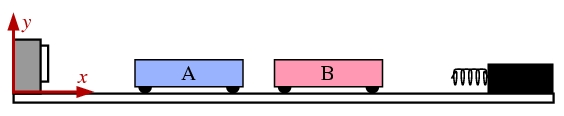
\includegraphics[scale=0.6]{Graphics/h6p7}
\end{center}

``In the experiment cart A rolls to the right on the level track, away from the motion sensor at the left end of the track. Cart B is initially at rest. The mass of cart A is equal to the mass of cart B. Suppose the two carts stick together after the collision. Assume the carts move frictionlessly.

The kinetic energy of the two carts after the collision:

(a) is equal to one half the kinetic energy of cart A before the collision.\\
(b) is equal to one quarter the kinetic energy of cart A before the collision.\\
(c) is equal to the kinetic energy of cart A before the collision.\\
(d) is equal to twice the kinetic energy of cart A before the collision.\\
(e) is equal to four times the kinetic energy of cart A before the collision.\\
(f) None of the above.''

Well, with no other source of energy, we can rule out options (d) and (e) at once. We should also be able to rule out (c) since this is an inelastic collision. However, let's do the math.

Momentum is conserved: $m_A v_A + m_B v_B = (m_A + m_B) v'$. However, $v_B = 0$, so

\begin{equation}
v' = \frac{m_A v_A}{m_A + m_B}
\end{equation}

The initial kinetic energy is

\begin{equation}
K = \frac{1}{2} m_A v_A^2
\end{equation}

while final kinetic energy is

\begin{equation}
K' = \frac{1}{2} (m_A + m_B) (v')^2 = \frac{1}{2} (m_A + m_B) \frac{m_A^2 v_A^2}{(m_A + m_B)^2} = \frac{m_A^2 v_A^2}{2(m_A + m_B)}
\end{equation}

The ratio between the two is $K'/K = \frac{m_A}{m_A + m_B}$. However, because $m_B = m_A$, we find that the kinetic energy is \emph{half} of the initial, the first choice.

\section{Problem 8: Man on cart throwing balls}

\begin{center}
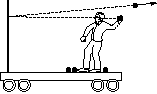
\includegraphics[scale=0.8]{Graphics/h6p8}
\end{center}

``Suppose you are on a cart, initially at rest on a track with very little friction. You throw balls at a partition that is rigidly mounted on the cart. If the balls bounce straight back as shown in the figure, is the cart put in motion?

(a) Yes, it moves to the right.\\
(b) Yes, it moves to the left.\\
(c) No, it remains in place.\\
(d) Not enough information is given to decide.''

The actual title of this problem is ``Man on throwing balls'', but I assume they simply missed the word ``cart''.

So this is an interesting problem. It's easy to say that the answer is obviously (c), given that it may appear that all forces are internal, which is in fact not the case. It would be the case if he caught the ball, but he doesn't!

As he throws a ball, it gains momentum towards the left, while he (and the cart, via friction in his shoes) gains momentum towards the right, so that momentum is conserved. Shortly thereafter, the ball bounces, and gives momentum to the cart towards the left, and the ball momentum to the right -- except that this change is \emph{twice as large} as when he throw the ball.\\
In throwing it, he changed the ball's momentum from $0$ to $m v$, while the bounce changed it from $m v$ to $-m v$, a change of $2 m v$. 

Defining the positive direction to be towards the left:\\
Before the throw, the cart and ball both have 0 momentum.\\
After the throw, the ball has momentum $m v$ and therefore the cart $- m v$, so that the sum is zero.\\
After the bounce, the ball has momentum $- m v$ and therefore the cart $+ m v$, so that, again, the sum is zero.

That's when the problem ends -- the ball exits the system, and the momentum is never cancelled out, so the cart gains a velocity towards the left.\\
If he caught the ball, we could add:\\
After the catch, the ball transfers its momentum $- m v$ to the cart, which then gets a momentum $m v - m v = 0$, and we are back where we began.

A simpler analysis:\\
Initial momentum of the system is zero, and final momentum of the ball is towards the right. That \emph{must} mean that there is an equal amount of momentum towards the \emph{left} of the cart, or momentum would not be conserved!

\section{Problem 9: Gravitational slingshot}

\begin{center}
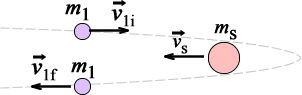
\includegraphics[scale=0.8]{Graphics/h6p9}
\end{center}

``A spacecraft of mass $m_1 = 4757$ kg with a speed $v_{1i} = \SI{3e3}{m/s}$ approaches Saturn which is moving in the opposite direction with a speed $v_s = \SI{9.6e3}{m/s}$. After interacting gravitationally with Saturn, the spacecraft swings around Saturn and heads off in the opposite direction it approached. The mass of Saturn is $m_s = \SI{5.69e26}{kg}$. Find the final speed $v_{1f}$ (in m/s) of the spacecraft after it is far enough away from Saturn to be nearly free of Saturn's gravitational pull.''

Spoiler alert: most of the text in this problem is justifying why the solution works, and is only necessary if you don't realize it at once. (I didn't, until it was ``too late'' to use the simple solution; I'd already solved it in more complex way.)

Considering the two as a system, there are no external forces, so momentum must be conserved. Momentum is a vector though, so we need to be careful with signs. If we take $v_{1i}$ to be positive, the initial velocity of Saturn is negative, and both velocities on the right-hand side are negative.

\begin{equation}
m_1 v_{1i} - m_s v_s = - m_1 v_{1f} - m_s v_{sf}
\end{equation}

We don't know $v_{1f}$ and we don't know $v_{sf}$ (the final velocity of Saturn). The latter must change, even if by an absolutely imperceptible amount.\\
With two unknowns, we need a second equation.\\
What more can we say and express as an equation? The total mechanical energy of the system should certainly be constant, since gravity is a conservative force. The mechanical energy here is

\begin{equation}
K_{m1} + U_{m1} + K_s + U_{s} = K'_{m1} + U'_{m1} + K'_s + U'_{s}
\end{equation}

Before we try to calculate this, which will clearly not be pretty, let's try to simplify it. Gravitational potential energy depends on two things: the two masses, and the distance between them. (Plus G, which is a constant, of course.) Therefore, if the problem starts and ends at the same distance $r$, or it starts and ends where $r$ is large enough that $U \approx 0$ (keep in mind that gravitational potential energy is always negative), we can assume that either that $U_{m1} = U'_{m1}$ and $U_s = U'_s$, or that all of those terms are practically zero. This simplifies things a great deal:

\begin{equation}
K_{m1} + K_s + = K'_{m1} + K'_s
\end{equation}

So now, the condition is that the sum of the kinetic energies are the same before and after, i.e. the increase in kinetic energy in the spacecraft comes from a decrease in Saturn's kinetic energy. 

With momentum and kinetic energy both conserved, we can solve this in a very simple way: this is an elastic collision. It doesn't matter that the force involved is gravity, instead of contact forces (that are mostly electromagnetic, in the end).

The mass of Saturn is about $10^{23}$ times greater than that of the satellite, so to an extremely good approximation, a reference frame centered on Saturn is the center of mass frame. For the same reason, the velocity of the COM frame is the velocity of Saturn -- the error here is so small that a pocket calculation would round it away entirely; in fact, I couldn't get Mathematica to give me an exact answer! All I can say is that it is much, much less than 1 nanometer per second, which it gives me for $m_1$ as large as $10^{11}$ kg. I think we'll be OK with this ``approximation''!

All we need to do, then, is transfer ourselves into the center of mass frame, by subtracting the center of mass velocity, find the velocity $u_{1f}$ (using $u$ instead of $v$ in the COM frame), and transfer back. We transfer into it by subtracting the COM velocity:

\begin{equation}
u_{1i} = v_{1i} - v_{cm} = v_{1i} - v_s = \SI{3e3}{m/s} + \SI{9.6e3}{m/s} = \SI{12.6e3}{m/s}
\end{equation}

Since Saturn's velocity is negative in our coordinate system, the subtraction becomes an addition. This makes sense, too: the center of mass, inside Saturn, sees the planets heading towards each other, so the net speed is larger than either of the individual speeds.

Next, we find the velocity after the collision. In the center of mass frame, this is just too easy: the signs flip. $u_{1f} = -u_{1i} = \SI{-12.6e3}{m/s}$.

Finally, we convert back to the reference frame of the outside observer by \emph{adding} the COM velocity of $\SI{-9.6e3}{m/s}$, and end up with

\begin{equation}
v_{1f} = u_{1f} + \SI{-9.6e3}{m/s} = -\SI{22.2e3}{m/s}
\end{equation}

They ask for the speed, though, so we need to drop the minus sign, and we are done.

\section{Problem 10: Railroad gun}

``A railroad gun of mass $M = 2.0$ kg fires a shell of mass $m = 1.0$ kg at an angle of $\theta = \ang{45}$ with respect to the horizontal as measured relative to the gun. After the firing is complete, the final speed of the projectile relative to the gun (muzzle velocity) is $v_0 = \SI{130.0}{m/s}$. The gun recoils with speed $v_r$ and the instant the projectile leaves the gun, it makes an angle $\phi$ with respect to the ground.

\begin{center}
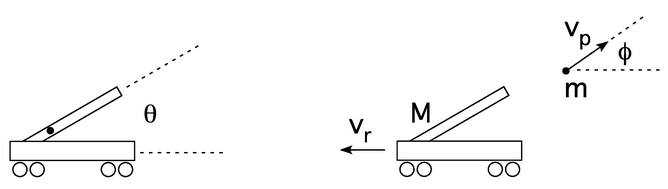
\includegraphics[scale=0.8]{Graphics/h6p10}
\end{center}

What is $v_p$, the speed of the projectile with respect to the ground (in m/s)?\\
What is $\phi$, the angle that the projectile makes with the horizontal with respect to the ground (in degrees)?''

I have to say that 2 kg for the entire gun and the car seems ridiculously low! If the projectile flies away at 130 m/s, via conservation of momentum, the rail car will move backwards with a speed of at least about a quarter of that (that's just guesswork), which is crazy fast, about the speed of a car on a freeway. I can't see it being less than a tenth, at least. I suppose we'll see soon enough.

Intuitively, I have to admit I thought $\phi = \theta$ and $v_p = v_0$, and thought of the recoil as separate thing, which is clearly not correct. Let's look at a proper analysis.

Clearly, conservation of momentum will be the main way we approach this problem.\\
Since this is a two-dimensional problem, there will be a bit more work than in the problems we've seen earlier on.

Momentum will be conserved in the $x$ direction, which will be quite a useful fact. What about the $y$ direction? Well, the shell clearly gains upwards momentum, but what about the car/gun? It is pushed down, but can't move downwards. Instead, the momentum is transferred to the Earth. After the launch, gravity acts on the shell, and so the $y$ component of its momentum will change.

Let's first think about this from the reference frame of the car. Not many strange things happen here: the shell launches at an angle $\theta$, and moves away from you at $v_0$ ($v_0 \cos \theta$ in the horizontal direction, and $v_0 \sin \theta$ upwards). So far, so good.

What happens according to an observer on the ground? The vertical component of the shell's motion is unchanged, since the car is stationary along the $y$ axis. In other words, this observer sees the shell move upwards at $v_0 \sin \theta$ m/s, same as someone on the car.\\
What about the horizontal component? I find it helpful to take things to extremes (even if they are unrealistic). What if the recoil speed of the car was greater than the shell's speed?\\
The horizontal component as seen from the ground would shrink, and since the vertical component is unchanged, the angle grows, and $v_p$ moves closer to $v_0 \sin \theta$.\\
This implies that $\phi > \theta$, and of course that $v_p < v_0$.

What about a more quantitative analysis? Let's first look at the reference frame of the rail gun. The equations for the shell is

\begin{align}
v_{0x} &= v_0 \cos \theta\\
v_{0y} &= v_0 \sin \theta
\end{align}

Nothing strange going on there.\\
In the reference frame of an outside observer, standing still on the ground, things change. Such an observer would see the gun speeding towards the left at the same time the shell starts flying to the right. To him, it is clear that the gunner would see the shell move \emph{faster} (in the x direction) than what he sees. In fact, in the limit where the speed of the gun and the speed of the shell are equal, the shell would move straight up to the outside observer.

The relevant equations here are also not very strange, but we can relate the two sets soon. First, the easy part:

\begin{align}
v_{px} &= v_p \cos \phi\\
v_{py} &= v_p \sin \phi
\end{align}

To the outside observer (and to the gunner), the rail gun is stationary along the y axis. Therefore, $v_0 \sin \theta = v_p \sin \phi$: the two agree on the vertical component. That gives us one useful relationship.

Next, we can relate the $x$ components. The difference there is a simple reference frame shift. As mentioned above, the outside observer sees the shell having a lower speed along the $x$ axis. The difference between the two frames is $v_r$.

\begin{equation}
v_p \cos \phi = v_0 \cos \theta - v_r
\end{equation}

Next, we can relate the momenta of the two objects. The initial momentum is zero, in both reference frames. Let's write a conservation equation in the outside frame.

\begin{equation}
m v_p \cos \phi - M v_r = 0
\end{equation}

Since $v_r$ is a speed in the opposite direction, we need a minus sign there. (Both terms will be positive, and their difference is zero.)

The final answer for $v_p$ has the form

\begin{equation}
v_p = (v_p \sin \phi) \hat{x} + (v_0 \sin \theta) \hat{y}
\end{equation}

... since the $y$ component is the same in both reference frames. However, we only need to find the $x$ component, and then calculate $\phi$ from that; so we don't really need to think of $\phi$ as an unknown, as far as solving the system goes. All we need is the $x$ component of the shell, as seen from the outside reference frame.

We have
\begin{equation}
m v_p \cos \phi - M v_r = 0
\end{equation}

But $v_p \cos \phi = (v_0 \cos \theta - v_r)$, so

\begin{align}
m (v_0 \cos \theta - v_r) - M v_r &= 0\\
m v_0 \cos \theta &= v_r(M + m)\\
\frac{m v_0 \cos \theta}{M + m} &= v_r
\end{align}

We know all of those variables, so we can find that $v_r = \SI{30.64129}{m/s}$. That means we can find the $x$ component:

\begin{equation}
v_{px} = v_0 \cos \theta - v_r = \SI{61.283}{m/s}
\end{equation}

We already had $v_{py}$ in terms of knowns, $v_0 \sin \theta$:

\begin{equation}
v_{py} = v_0 \sin \theta = \SI{91.9239}{m/s}
\end{equation}

We can then finally find $v_p$ and the angle $\phi$:

\begin{align}
v_p  &= \sqrt{v_{px}^2 + v_{py}^2} = \SI{110.479}{m/s}\\
\phi &= \arctan \frac{v_{py}}{v_{px}} = \ang{56.31}
\end{align}

\end{document}